\documentclass{book}
\usepackage[full]{leadsheets}
\usepackage[a4paper, margin=0.75in]{geometry}
\usepackage{multicol}
\usepackage[polish]{babel}
\usepackage{array}
\usepackage{graphicx}
\thispagestyle{empty}

%\usepackage[default]{lato}
%\usepackage[T1]{fontenc}

\selectlanguage{polish}
\DeclareTranslation{Polish}{leadsheets/chorus}{Ref.}
\DeclareTranslation{Polish}{leadsheets/lyrics}{tekst}
\DeclareTranslation{Polish}{leadsheets/verse}{Zwr.}

\definesongtitletemplate{custom}{%
    \section*{\songproperty{title}}%
    \ifsongproperty{music}{%
        \begingroup\footnotesize
            Muzyka: \songproperty{music}
        \endgroup
    }{}%
}

\setleadsheets{title-template = custom}

\begin{document}

\begin{titlepage}
    \begin{center}
        \vspace*{7cm}
        
        %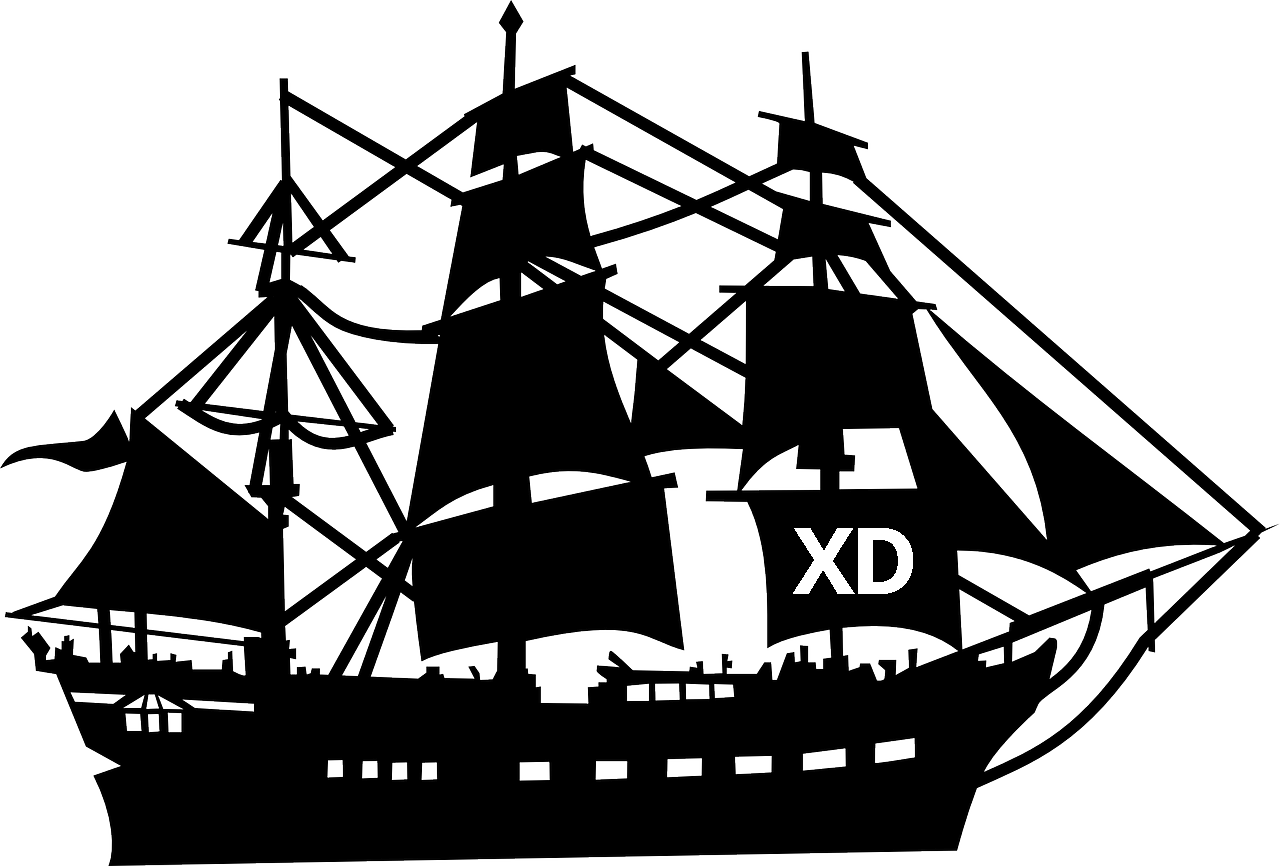
\includegraphics[width=0.75\textwidth]{front-obrazek.png}
        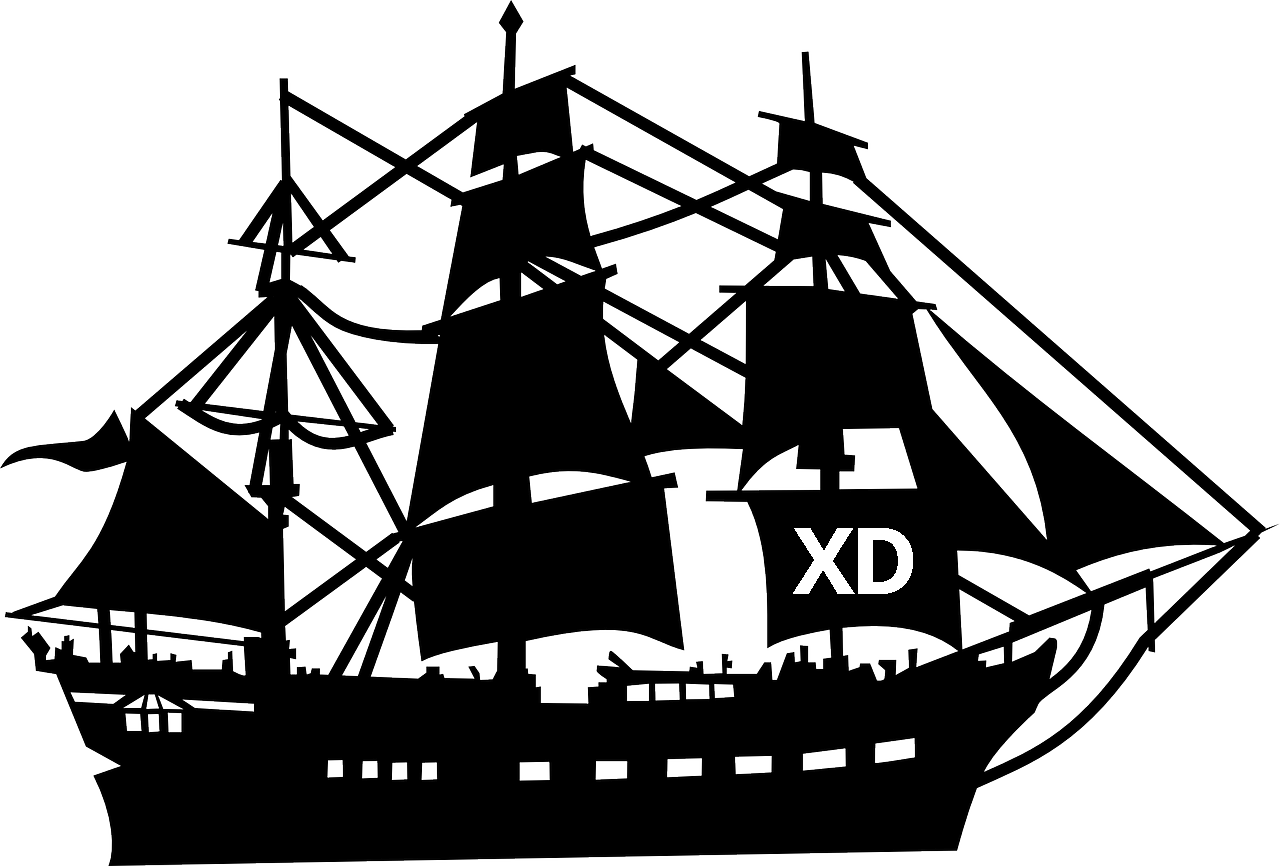
\includegraphics[height=8cm]{front-obrazek.png}

        \vspace{1cm}

        \Huge\textbf{Jakieś piosenki}

        \vspace{0.5cm}

        \LARGE{może szanty}

        \vfill

        \Large
        Wydawnictwo Kis Inkris \\
        Warszawa, 2021
    \end{center}
\end{titlepage}

\begin{song}[verse/numbered, remember-chords, align-chords={l}]{title={Kapitan Kidd}, music={North Cape}}
\begin{multicols}{2}
    \begin{chorus}
        Me ^{e}imię ^{h}William ^{e}Kidd \\
        Już czeka ^{a}stryk, czeka ^{D}stryk \\
        Królewski ^{e}korsarz ^{h}William ^{e}Kidd, czeka ^*{G}stry ^{D}k \\
        Me ^{G}imię ^{D}William ^{a}Kidd \\
        Zbrodni ^*{e}ogrom ^{h}nych to ^{a}mit \\
        Powró^{e}ciłem, ^{G}choć w Lon^{h}dynie ^{D/F#}czeka ^{e}stryk
    \end{chorus}
    \begin{verse}
        Mój ^{e}ojciec ^{h}uczył ^{e}mnie \\
        Jak nie ^{G}znaleźć się na ^{D}dnie \\
        Lecz los o^{e}krutny ^{D}zabrał ^{a}go ro^{h}dzinie ^{e}mej \\
        Choć biblię w ^{e}rękę ^{h}moją ^{e}kładł \\
        Morza ^{G}urok na mnie ^{D}padł \\
        I mary^{e}narzem ^{D}stałem ^{a}się, choć ^{h}czeka ^{e}stryk
    \end{verse}
    \begin{chorus}
        Me imię William Kidd\ldots
    \end{chorus}
    \begin{verse}
        Kanonier William Moore \\
        Pierwszy trafił na mój sznur \\
        Bo przeciw mnie ośmielił się on wzniecić bunt \\
        Choć dobrym strzelcem William był \\
        Pod salingiem będzie gnił \\
        Buntownik każdy skończy tak, już czeka stryk
    \end{verse}
    \begin{chorus}
        Me imię William Kidd\ldots
    \end{chorus}
    \begin{verse}
        Raz gdy było ze mną źle \\
        Obiecałem sobie, że \\
        Mądrości drogą odtąd pójdę po kres dni \\
        Lecz mój korsarski podły fach \\
        Zabił wnet o duszę strach \\
        I potępienie czeka mnie, bo czeka stryk
    \end{verse}
    \begin{chorus}
        Me imię William Kidd\ldots
    \end{chorus}
    \begin{verse}
        \textit{(wolniej)} \\
        To egzekucyjny blok \\
        Zaraz mnie ogarnie mrok \\
        Bo na mą szyję kat założy gruby sznur \\
        Więc dzisiaj ostrzec ciebie chcę \\
        Byś za przykład nie brał mnie \\
        Mądrości drogą zawsze szedł, bo czeka stryk
    \end{verse}
    \begin{chorus}
        \textit{(szybciej)} \\
        Me imię William Kidd\ldots
    \end{chorus}
\end{multicols}
\end{song}


\end{document}
